%%%%%%%%%%%%%%%%%%%%%%%%%%%%%%%%%%%%%%%%
% Jacobs Landscape Poster
% LaTeX Template
% Version 1.1 (14/06/14)
%
% Created by:
% Computational Physics and Biophysics Group, Jacobs University
% https://teamwork.jacobs-university.de:8443/confluence/display/CoPandBiG/LaTeX+Poster
%
% Further modified by:
% Nathaniel Johnston (nathaniel@njohnston.ca)
%
% This template has been downloaded from:
% http://www.LaTeXTemplates.com
%
% License:
% CC BY-NC-SA 3.0 (http://creativecommons.org/licenses/by-nc-sa/3.0/)
%
%%%%%%%%%%%%%%%%%%%%%%%%%%%%%%%%%%%%%%%%%

%----------------------------------------------------------------------------------------
%	PACKAGES AND OTHER DOCUMENT CONFIGURATIONS
%----------------------------------------------------------------------------------------

\documentclass[final]{beamer}

\usepackage[scale=1.24]{beamerposter} % Use the beamerposter package for laying out the poster
\usepackage{subcaption}
\usepackage{blkarray}

\usetheme{confposter} % Use the confposter theme supplied with this template

\newcommand{\psrsigma}{\langle \Sigma, \aone, \ainf, \{\A_\sigma\}_{\sigma \in \Sigma} \rangle}
\newcommand{\mpsrsigma}{\langle \Sigma, \Sigma', \kappa, \aone, \ainf, \{\A_\sigma\}_{\sigma \in \Sigma'} \rangle}

\setbeamercolor{block title}{fg=black,bg=white} % Colors of the block titles
\setbeamercolor{block body}{fg=black,bg=white} % Colors of the body of blocks
\setbeamercolor{block alerted title}{fg=white,bg=ddblue!70} % Colors of the highlighted block titles
\setbeamercolor{block alerted body}{fg=black,bg=dblue!10} % Colors of the body of highlighted blocks
% Many more colors are available for use in beamerthemeconfposter.sty

%-----------------------------------------------------------
% Define the column widths and overall poster size
% To set effective sepwid, onecolwid and twocolwid values, first choose how many columns you want and how much separation you want between columns
% In this template, the separation width chosen is 0.024 of the paper width and a 4-column layout
% onecolwid should therefore be (1-(# of columns+1)*sepwid)/# of columns e.g. (1-(4+1)*0.024)/4 = 0.22
% Set twocolwid to be (2*onecolwid)+sepwid = 0.464
% Set threecolwid to be (3*onecolwid)+2*sepwid = 0.708

\newlength{\sepwid}
\newlength{\onecolwid}
\newlength{\twocolwid}
\newlength{\threecolwid}
\setlength{\paperwidth}{48in} % A0 width: 46.8in
\setlength{\paperheight}{36in} % A0 height: 33.1in
\setlength{\sepwid}{0.024\paperwidth} % Separation width (white space) between columns
\setlength{\onecolwid}{0.22\paperwidth} % Width of one column
\setlength{\twocolwid}{0.464\paperwidth} % Width of two columns
\setlength{\threecolwid}{0.708\paperwidth} % Width of three columns
\setlength{\topmargin}{-0.5in} % Reduce the top margin size
%-----------------------------------------------------------

\usepackage{graphicx}  % Required for including images

\usepackage{booktabs} % Top and bottom rules for tables


\newcommand{\dist}{\mathsf{dist}}
%\newcommand{\mathbold}[1]{\boldsymbol{#1}}

% Definition of oracles
\newcommand{\oracle}[1]{\mathsf{#1}}
\newcommand{\SQ}{\oracle{SQ}}
\newcommand{\SQD}{\oracle{SQ}^D}
\newcommand{\SQT}{\oracle{SQ}^T}
\newcommand{\EX}{\oracle{EX}}
\newcommand{\DIFF}{\oracle{DIFF}_\infty^D}
\newcommand{\DIFFT}{\oracle{DIFF}_\infty^T}

% Sets with name
\newcommand{\sstar}{\Sigma^\star}
\newcommand{\Sstar}{\sstar}
%\renewcommand{\R}{\mathbb{R}}
\newcommand{\R}{\mathbb{R}}

% Definition of algorithms
\newcommand{\algoname}[1]{\texttt{\upshape #1}}
\newcommand{\CT}{\algoname{CT}}
\newcommand{\CTS}{\algoname{CT}_{\SQ}}
\newcommand{\CTLS}{\algoname{CT}_{\Linf,\SQ}}
\newcommand{\Learner}{\algoname{L}}
\newcommand{\adaptive}{\algoname{ParameterSearch}}
\newcommand{\chgdet}{\algoname{ChangeDetector}}
\newcommand{\basic}{\algoname{StreamLearner}}
\newcommand{\sm}{\basic}
\newcommand{\spsv}{\algoname{SpSv}}
\newcommand{\prespsv}{\algoname{SpSv}^{\mathrm{p}}}
\newcommand{\pss}{\prespsv}
\newcommand{\stest}{\algoname{SIMILARITY-TEST}}
\newcommand{\test}{\algoname{Test}}
\newcommand{\estimate}{\algoname{Estimate}}
\newcommand{\whileloop}{\algoname{while}}
\newcommand{\sketch}{\algoname{Sketch}}
\newcommand{\skinsert}{\algoname{Sketch.insert}}
%\newcommand{\algo}{\mathsf{HMC\!+\!SM}}
%\newcommand{\algopl}{\mathsf{HMC_{p,\ell}\!+\!SM}}
\newcommand{\algo}{\texttt{HMC+SM}}
\newcommand{\algopl}{\texttt{\upshape HMC}_{p,\ell}\texttt{\upshape +SM}}

% Constants used in algorithms
\newcommand{\requal}{\algoname{equal}}
\newcommand{\rdistinct}{\algoname{distinct}}
\newcommand{\rnotclear}{\algoname{not clear}}
\newcommand{\runknown}{\algoname{unknown}}

% Definition of constats
\newcommand{\constantsym}[1]{\texttt{\upshape `#1'}}
\newcommand{\QM}{\constantsym{?}}
\newcommand{\Ms}{M_{\mathrm s}}
\newcommand{\Ts}{T_{\mathrm s}}
\newcommand{\Tt}{T_{\mathrm t}}
\newcommand{\Nu}{N_{\mathrm u}}
\newcommand{\Ne}{N_{\mathrm e}}
\newcommand{\NExp}{N_{\mathrm E}}
\newcommand{\Nd}{N_{\mathrm d}}
\newcommand{\Nl}{N_{\mathrm l}}
\newcommand{\Nt}{N_{\mathrm t}}
\newcommand{\Nx}{N_{\mathrm x}}
\newcommand{\Te}{T_{\mathrm e}}
\newcommand{\Fs}{F_{\mathrm s}}
\newcommand{\Fsc}{\bar{F}_{\mathrm s}}
\newcommand{\Ft}{F_{\mathrm t}}
\newcommand{\Fw}{F_{\mathrm w}}
\newcommand{\Fwc}{\bar{F}_{\mathrm w}}
\newcommand{\Us}{U_{\mathrm s}}
\newcommand{\Ut}{U_{\mathrm t}}
\newcommand{\Qf}{Q_{\mathrm f}}
\newcommand{\Qfp}{Q'_{\mathrm f}}
\newcommand{\epss}{\varepsilon_{\mathrm s}}
\newcommand{\epst}{\varepsilon_{\mathrm t}}
\newcommand{\epse}{\varepsilon_{\mathrm e}}
\newcommand{\epsg}{\varepsilon_{\mathrm g}}
\newcommand{\epsx}{\varepsilon_{\mathrm x}}

% Definition of classes
\newcommand{\fclass}[1]{\mathcal{#1}}
\newcommand{\PDFA}{\fclass{PDFA}}
\newcommand{\GPDFA}{\fclass{GPDFA}}
\newcommand{\WFA}{\fclass{WFA}}
%\newcommand{\qPDFA}{\widetilde{\fclass{PDFA}}}
%\renewcommand{\lang}[1]{\mathcal{L}(#1)}
\newcommand{\lang}[1]{\mathcal{L}(#1)}
%\newcommand{\Exp}{\mathrm{Exp}}
\newcommand{\Exp}{\operatorname{Exp}}

% Definition of statistical operators
\newcommand{\statistic}[1]{\mathbb{#1}}
%\renewcommand{\E}{\statistic{E}}
\newcommand{\E}{\statistic{E}}
\newcommand{\Emp}{\hat{\statistic{E}}}
\renewcommand{\P}{\statistic{P}}
\newcommand{\V}{\statistic{V}}
\newcommand{\Lik}{\statistic{L}}
\newcommand{\LLik}{\statistic{LL}}

% Definition of L distances
%\newcommand{\Ldist}{\mathrm{L}}
\newcommand{\Ldist}{\operatorname{L}}
\newcommand{\Linf}{\Ldist_\infty}
\newcommand{\evnt}[1]{\mathfrak{#1}}
\newcommand{\eA}{\evnt{E}}
\newcommand{\eB}{\evnt{X}}
\newcommand{\LinfA}{\Ldist_\infty^{\eA}}
\newcommand{\LinfAn}{\Ldist_\infty^{\eA_n}}
\newcommand{\LinfB}{\Ldist_\infty^{\eB}}
\newcommand{\Lone}{\Ldist_1}
\newcommand{\Ltwo}{\Ldist_2}
\newcommand{\prefLinf}{\Ldist_\infty^{\mathrm{p}}}
%\newcommand{\KL}{\mathrm{KL}}
\newcommand{\KL}{\operatorname{KL}}
\newcommand{\scLinf}{\textsc{l}_{\scriptscriptstyle \infty}}
%%% MAIN OR PRESS
\newcommand{\scprefLinf}{\textsc{l}_\infty^{\normalfont\textrm{\bfseries\tiny{p}}}}
%\newcommand{\scprefLinf}{\textsc{l}_{\scriptscriptstyle \mathbold{\infty}}^{\normalfont\textrm{\fontseries{b}\fontsize{4}{4}\selectfont p}}}

% Definition of norms
\newcommand{\norm}[1]{\|#1\|}
\newcommand{\frob}[1]{\norm{#1}_F}
\newcommand{\lone}[1]{\norm{#1}_1}
\newcommand{\ltwo}[1]{\norm{#1}_2}
\newcommand{\linf}[1]{\norm{#1}_\infty}
\newcommand{\lp}[1]{\norm{#1}_p}
\newcommand{\Lp}{\ell_p}

% Definition of mathematical operators
% Supremum
\DeclareMathOperator{\supp}{supp}
% Indicator function
\newcommand{\one}{\mathbb{I}}
% Longest common prefix
\DeclareMathOperator{\lcp}{lcp}
% Set of all prefixes
\DeclareMathOperator{\pref}{pref}
% Trace
\DeclareMathOperator{\tr}{tr}
% Vector
\DeclareMathOperator{\matvec}{vec}
%
\DeclareMathOperator{\shr}{shr}

% Definition of mathematical environments
%\newtheoremstyle{theoremsc}%
%{\topsep}%
%{\topsep}%
%{\itshape}%
%{0pt}%
%{\scshape\bfseries}%
%{.}%
%{5pt plus 1pt minus 1pt}%
%{}
%%\newtheoremstyle{plain}
%%  {\topsep}   % ABOVESPACE
%%  {\topsep}   % BELOWSPACE
%%  {\itshape}  % BODYFONT
%%  {0pt}       % INDENT (empty value is the same as 0pt)
%%  {\bfseries} % HEADFONT
%%  {.}         % HEADPUNCT
%%  {5pt plus 1pt minus 1pt} % HEADSPACE
%%  {}          % CUSTOM-HEAD-SPEC
%\theoremstyle{theoremsc}
%\newtheorem{theorem}{Theorem}
%\newtheorem{lemma}[theorem]{Lemma}
%\newtheorem{definition}[theorem]{Definition}
%%\newtheorem{claim}[theorem]{Claim}
%\newtheorem{corollary}[theorem]{Corollary}
%\newtheorem{proposition}[theorem]{Proposition}
%%\newtheorem{assumptions}{Assumption}{\bfseries}{\upshape}
%\newtheorem{assumptions}{Assumption}
%\newtheorem{assumption}{Assumption}
%%\newtheorem{assumptions*}{Assumptions}
%%\spnewtheorem*{assumptions*}{Assumptions}{\bfseries}{\upshape}
%%\spnewtheorem{claim}{Claim}{\bfseries}{\upshape}
%\theoremstyle{remark}
%%\newtheorem{claim}[section]{Claim}
%%\newtheorem{remark}[section]{Remark}
%%\newtheorem{claim}{Claim}[chapter]
%%\newtheorem{remark}{Remark}[chapter]

% Marker for copy-and-paste text
\newcommand{\copytext}{\noindent \rule{\textwidth}{1pt}\\ \texttt{COPY COPY COPY COPY COPY COPY COPY COPY COPY COPY COPY COPY}\\ \rule{\textwidth}{1pt}\\} 

% Imported directly from NIPS12
\newcommand{\Rset}{\mathbb{R}}
\newcommand{\Nset}{\mathbb{N}}
\newcommand{\Hset}{\mathbb{H}}

\DeclareMathOperator*{\argmax}{\rm argmax}
\DeclareMathOperator*{\argmin}{\rm argmin}
\DeclareMathOperator{\sgn}{sgn}
\DeclareMathOperator{\sign}{sign}
\DeclareMathOperator{\range}{range}
\DeclareMathOperator{\rank}{rank}
\DeclareMathOperator{\diag}{diag}
\DeclareMathOperator{\local}{local}
\DeclareMathOperator{\Tr}{Tr}
\providecommand{\frobp}[2]{\langle#1, #2\rangle_F}

\newcommand{\set}[1]{\{#1\}}
\newcommand{\iprod}[2]{\left\langle #1 , #2 \right\rangle}
%%% MAIN OR PRESS
\newcommand{\mat}[1]{\mathbf{#1}}
%\newcommand{\mat}[1]{\mathbold{#1}}
\newcommand{\A}{\mat{A}}
\newcommand{\B}{\mat{B}}
\newcommand{\M}{\mat{M}}
\renewcommand{\H}{\mat{H}}

\newcommand{\h}{\hat}
\newcommand{\tl}{\tilde}
\newcommand{\Bs}{\mathcal{B}}
\newcommand{\cB}{\Bs}
%\newcommand{\cD}{\mathcal{D}}
\newcommand{\cD}{D}
\newcommand{\Ps}{\mathcal{P}}
\newcommand{\Ss}{\mathcal{S}}
\newcommand{\cW}{\mathcal{W}}
\newcommand{\Vsv}{\mat{V}}

\newcommand{\RempSt}{\hat{R}_{\tilde{S}}}
\newcommand{\RempStp}{\hat{R}_{\tilde{S}'}}
\newcommand{\RempS}{\hat{R}_{S}}
\newcommand{\hrt}{\mat{h}_{\lambda,\Ss}^\top}
\newcommand{\hr}{\mat{h}_{\lambda,\Ss}}
\newcommand{\hc}{\mat{h}_{\Ps,\lambda}}
\newcommand{\hhrt}{\hat{\mat{h}}_{\lambda,\Ss}^\top}
\newcommand{\hhr}{\hat{\mat{h}}_{\lambda,\Ss}}
\newcommand{\hhc}{\hat{\mat{h}}_{\Ps,\lambda}}

%%% MAIN OR PRESS
\newcommand{\pivec}{\boldsymbol{\pi}}
\newcommand{\alphavec}{\boldsymbol{\alpha}}
\newcommand{\thetavec}{\boldsymbol{\theta}}
\newcommand{\vectheta}{\thetavec}
\newcommand{\vecalpha}{\alphavec}
\newcommand{\rhovec}{\boldsymbol{\rho}}
\newcommand{\vecrho}{\rhovec}
\newcommand{\aone}{\boldsymbol{\alpha}_\lambda}
%\newcommand{\aone}{\boldsymbol{\alpha}_0}
\newcommand{\ainf}{\boldsymbol{\alpha}_{\infty}}
\newcommand{\taone}{\tilde{\boldsymbol{\alpha}}_0}
\newcommand{\tainf}{\tilde{\boldsymbol{\alpha}}_{\infty}}
\newcommand{\haone}{\hat{\boldsymbol{\alpha}}_0}
\newcommand{\hainf}{\hat{\boldsymbol{\alpha}}_{\infty}}
\newcommand{\bone}{\boldsymbol{\beta}_0}
\newcommand{\binf}{\boldsymbol{\beta}_{\infty}}
\newcommand{\vecb}{\boldsymbol{\beta}}
\newcommand{\tbone}{\tilde{\boldsymbol{\beta}}_0}
\newcommand{\tbinf}{\tilde{\boldsymbol{\beta}}_{\infty}}
\newcommand{\hbone}{\hat{\boldsymbol{\beta}}_0}
\newcommand{\hbinf}{\hat{\boldsymbol{\beta}}_{\infty}}
%\newcommand{\aone}{\mathbold{\alpha}_0}
%\newcommand{\ainf}{\mathbold{\alpha}_{\infty}}
%\newcommand{\taone}{\tilde{\mathbold{\alpha}}_0}
%\newcommand{\tainf}{\tilde{\mathbold{\alpha}}_{\infty}}
%\newcommand{\haone}{\hat{\mathbold{\alpha}}_0}
%\newcommand{\hainf}{\hat{\mathbold{\alpha}}_{\infty}}
%\newcommand{\bone}{\mathbold{\beta}_0}
%\newcommand{\binf}{\mathbold{\beta}_{\infty}}
%\newcommand{\tbone}{\tilde{\mathbold{\beta}}_0}
%\newcommand{\tbinf}{\tilde{\mathbold{\beta}}_{\infty}}
%\newcommand{\hbone}{\hat{\mathbold{\beta}}_0}
%\newcommand{\hbinf}{\hat{\mathbold{\beta}}_{\infty}}

\newcommand{\Alpha}{\aone}
\newcommand{\Beta}{\ainf}
\newcommand{\psrA}{\mathcal{A}}
\newcommand{\wa}{\langle  \aone, \ainf, \{\A_\sigma\} \rangle}
\newcommand{\wasigma}{\langle  \aone, \ainf, \{\A_\sigma\}_{\sigma \in \Sigma} \rangle}
\newcommand{\wb}{\langle  \bone, \binf, \{\B_\sigma\} \rangle}
\newcommand{\wap}{\langle  \aone', \ainf', \{\A'_\sigma\} \rangle}
\newcommand{\wbp}{\langle  \bone', \binf', \{\B'_\sigma\} \rangle}
\newcommand{\wat}{\langle  \taone, \tainf, \{\tilde{\A}_\sigma\} \rangle}
\newcommand{\wtt}{\langle  \taone, \tainf, \{\tilde{\A}_\sigma^\delta\} \rangle}
\newcommand{\wt}{\langle  \aone, \ainf, \{{\A}_\sigma^\delta\} \rangle}
\newcommand{\wbt}{\langle  \tbone, \tbinf, \{\tilde{\B}_\sigma\} \rangle}
\newcommand{\wah}{\langle  \haone, \hainf, \{\hat{\A}_\sigma\} \rangle}
\newcommand{\wbh}{\langle  \hbone, \hbinf, \{\hat{\B}_\sigma\} \rangle}
\newcommand{\mdp}{\langle  S, A, P, R \rangle}
\newcommand{\mdpoptomega}{\langle  I_\omega, \pi_\omega, \beta_\omega \rangle}
\newcommand{\mdpopt}{\langle  I, \pi, \beta \rangle}
\newcommand{\optmodS}{\langle  \vecalpha, \mat{1}, \{\A_\sigma\}_{\sigma \in \Sigma} \rangle}
\newcommand{\optmod}{\langle  \vecalpha, \mat{1}, \{\A_\sigma\} \rangle}

\newcommand{\erho}{\epsilon_\rho}
\newcommand{\eP}{\epsilon_P}
\newcommand{\sO}{\sigma_O}
\newcommand{\sP}{\sigma_P}
\newcommand{\sval}{\mathfrak{s}}

\newcommand{\loss}{\ell}
\newcommand{\cvloss}{\tilde{\ell}}

% From ICML12
\newcommand{\U}{\mathcal{U}}
\newcommand{\spn}{\operatorname{span}}

\newcommand\scalemath[2]{\scalebox{#1}{\mbox{\ensuremath{\displaystyle #2}}}}

%----------------------------------------------------------------------------------------
%	TITLE SECTION
%----------------------------------------------------------------------------------------

\title{Learning Multi-Step Predictive
     State Representations} % Poster title

\author{Lucas Langer, Borja Balle, Doina Precup} % Author(s)

\institute{Reasoning and Learning Lab, McGill University} % Institution(s)

%----------------------------------------------------------------------------------------

\begin{document}

\addtobeamertemplate{block end}{}{\vspace*{2ex}} % White space under blocks
\addtobeamertemplate{block alerted end}{}{\vspace*{2ex}} % White space under highlighted (alert) blocks

\setlength{\belowcaptionskip}{2ex} % White space under figures
\setlength\belowdisplayshortskip{2ex} % White space under equations

\begin{frame}[t] % The whole poster is enclosed in one beamer frame

\begin{columns}[t] % The whole poster consists of three major columns, the second of which is split into two columns twice - the [t] option aligns each column's content to the top

\begin{column}{\sepwid}\end{column} % Empty spacer column

\begin{column}{\onecolwid} % The first column

%----------------------------------------------------------------------------------------
%	OBJECTIVES
%----------------------------------------------------------------------------------------

\begin{block}{Abstract}
With spectral learning algorithms, we consider the problem of making predictions in partially observable environments. Spectral algorithms learn a linear representation of a system's internal states and can be used to make predictions of future observations conditioned on the past. Such predictions have been applied to robotics, where expectations of the future guide planning decisions (Pierre Luc). 
%They can also be used in medical time-series, such as when one has evolving information from a patient (blood sugar, temperature, etc.) and wants to assess the health of the patient. 
Spectral algorithms have the advantage that they are statistically consistent with well known error bounds (Citation). In this work, we develop a novel extension to a previous spectral based representation. We augment Predictive State Representations (PSRs) with multi-step transition operators to get Multi-Step Predictive State Representations (M-PSRs). In experiments, the novel representation far outperforms its predecessor when using regularized models.

\end{block} 
 
%\begin{block}{Highlights}
%We considered the problem of making predictions in %partially observable environments with spectral learning %algorithms:

%\begin{itemize}
%\item Based on previous work with predictive state %representations (PSR), we developed a novel extension %called the M-PSR
%\item We developed algorithms for learning the new %parameters  of M-PSRs
%\item We applied M-PSRs to robot navigation in labyrinth %environments and found large performance improvements
%\end{itemize}
%\end{block}

%----------------------------------------------------------------------------------------
%	INTRODUCTION
%----------------------------------------------------------------------------------------

%\begin{block}{Motivation}

%Spectral algorithms have theoretical guarantees which make them highly desirable to use over other methods. Traditional applications of such models include:

%\begin{itemize}
%  \item Planning decisions in robotics or game AIs
%  \item Natural language processing
%  \item Time series: medical data, speech processing, %financial modelling)
%\end{itemize}

%\end{block}

\begin{block}{Overview}

\begin{figure}
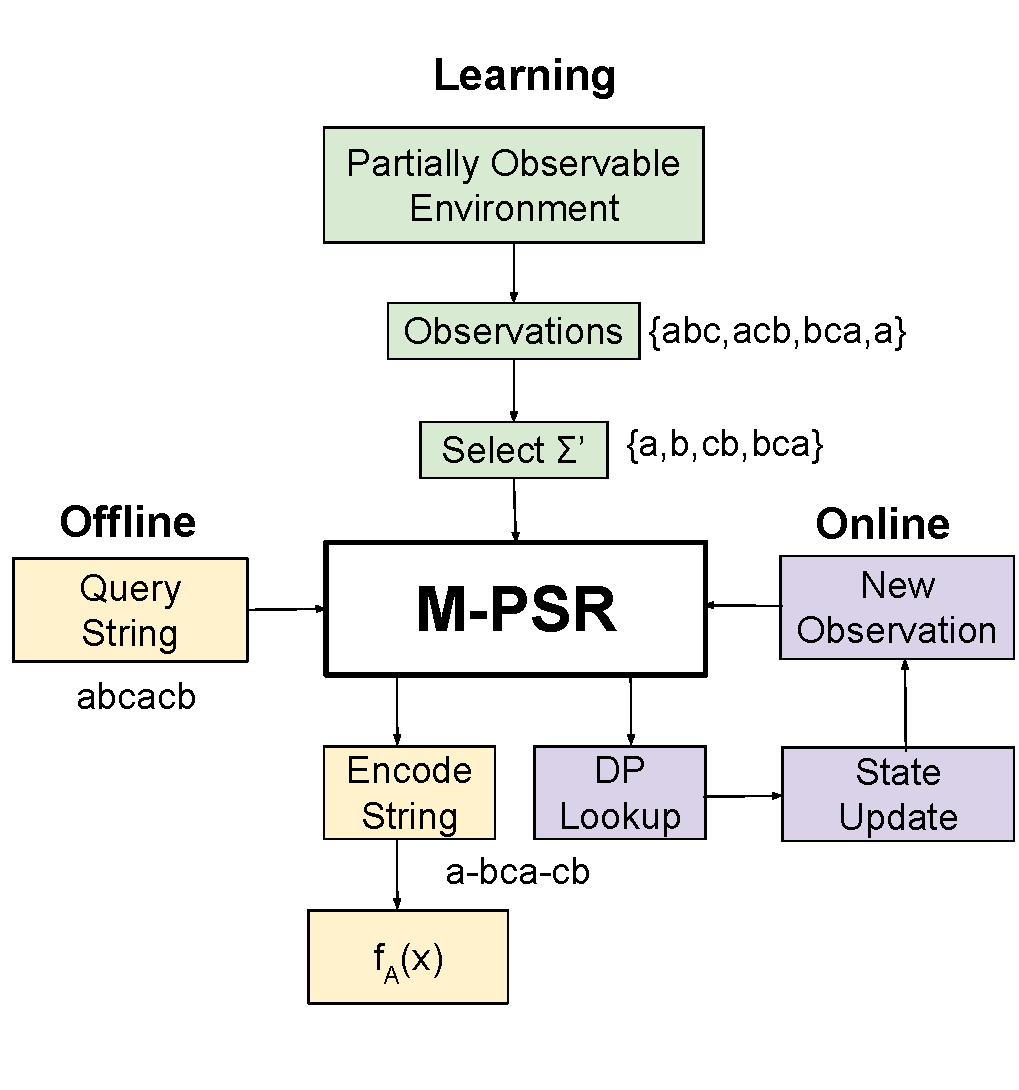
\includegraphics[height=33cm,width=1.00\linewidth]{M-PSR_Flow_Chart.pdf}
\end{figure}

\end{block}





%----------------------------------------------------------------------------------------

\end{column} % End of the first column
\begin{column}{\sepwid}\end{column} % Empty spacer column
\begin{column}{\twocolwid} % Begin a column which is two columns wide (column 2)
\begin{columns}[t,totalwidth=\twocolwid] % Split up the two columns wide column

\begin{column}{\twocolwid}\vspace{-.6in} % The first column within column 2 (column 2.1)

\begin{block}{Multi-Step Predictive State Representations (M-PSRs)}

As with traditional PSRs, M-PSRs compute a probability function  on observation strings $f_A: \Sigma^{*} \mapsto [0,1]$. 
A traditional PSR is defined by the tuple: $\psrsigma$, where $\Sigma$ is the set of observations, $\alpha_{\lambda}$ is an initial weighting on states, $\alpha_{\infty}$ is a normalizing vector, and $\{\A_\sigma\}_{\sigma \in \Sigma}$ is a set of transition operators.
%We define an M-PSR by the tuple: $\mpsrsigma$. 
%The goal of the
An M-PSR expresses transitions more compactly
%. This is accomplished 
by including operators which represent sequences of observations: $\Sigma' \subset \Sigma^*$
%.   With additional operators, it becomes necessary to specify
and a way of partitioning strings
%. For an M-PSR, we call this it's 
which we call an encoding function $\kappa$.

\end{block}

\begin{block}{Probability Queries}

%To illustrate the difference between PSRs and M-PSRs, we will show probability queries using both representations. 
With traditional PSRs, transition operators are applied for each observation $\sigma_i$ in $x=\sigma_1 \cdots \sigma_n$.

\begin{equation*}
f_{\psrA}(x) ~=~ f_{\psrA}(\sigma_1 \cdots \sigma_n) ~=~ \aone^\top \A_{\sigma_1} \cdots \A_{\sigma_n} \ainf ~=~ \aone^\top \A_x \ainf \enspace.
\end{equation*}


For M-PSRs, we apply multi-step transition operators for each observation sequence $s_i$ in $\kappa(x)=s_1 \cdots s_m$

%Here, m is the length of the encoding and depends on x.

\begin{equation*}
f_{\psrA}(x) ~=~ f_{\psrA}(s_1 \cdots s_m) ~=~ \aone^\top \A_{s_1} \cdots \A_{s_m} \ainf ~=~ \aone^\top \A_x \ainf \enspace.
\end{equation*}

%One can also perform conditional queries, which are necessary for applications such as planning where one wishes to predict the future given the past.

%\begin{equation*}
%f_{\psrA}(x|y) = \frac{\aone^\top \A_x \ainf}{\aone^\top %\A_y \ainf} \enspace.
%\end{equation*}

\end{block}
\end{column} % End of column 2.2
\end{columns} % End of the split of column 2 - any content after this will now take up 2 columns width


%\begin{block}{Learning M-PSRs from Data}

%The probabilities over sequences in our embedded system can be summarized in a Hankel matrix,
%a bi-infinite (conceptually) matrix $\H_f \in \R^{\Sstar \times \Sstar}$ with rows and
%columns indexed by strings in $\Sstar$. We estimated the Hankel matrix for a fixed finite subsets of rows and columns. The SVD decomposition
%of $\H_f$ provides a way to recover a PSR (see Boots et al., 2011). This algorithm is easily extended for M-PSRs and remains statistically consistent.

%\end{block}

\begin{block}{Base M-PSRs}

As an example, a natural approach to build an M-PSR for timing $\Sigma=\{\sigma\}$, is to use powers of a fixed base $b$:

\begin{equation*}
\Sigma' ~=~ \{\sigma,~\sigma^b,~ \sigma^{b^2},\ldots, \sigma^{b^K}\}
\end{equation*}

For given observation string: $\sigma^t$, we compute $t = t_0 b^0 + t_1 b^1 + t_2 b^2 + \cdots + t_K b^K$ and then the encoding follows:

\begin{equation*}
\kappa(\sigma^t) ~=~ (\sigma^{b^K})^{t_K}~ (\sigma^{b^{K-1}})^{t_{K-1}} \cdots (\sigma^b)^{t_1}~ (\sigma)^{t_0}
\end{equation*}

%, where $0 \leq t_k \leq b - 1$ for $0 \leq k \leq K$, and $t_K \geq 0$

\end{block}

\begin{block}{Data-Driven M-PSRs}

%Experiments indicate that compact representations of transitions yield better predictions.

For a general M-PSR we propose that $\kappa(x)$ be the encoding of minimal length. $\kappa(x)$ is computed by dynamic programming, giving the additional benefit that one can perform optimal state updates for online applications. 

\begin{equation*}
\kappa(x) ~= \argmin_{ z \in \Sigma^*, \; x=yz, \; |y|<|x|} |~\kappa(y)(z)| \enspace 
\end{equation*}

With this choice of $\kappa$, we build $\Sigma'$ by iteratively selecting sub-strings from the training set:

\begin{equation*}
\Sigma'_{i+1} ~=~ \argmin_{u \in \mathrm{sub}_M} ~\sum_{x \in \mathrm{train}} |\kappa_{\Sigma_i' \cup \{u\}}(x)| \enspace
\end{equation*}

% Is y supposed to be in \Sigma* here???
%Above, $\partial$ is the decoding function for $\kappa$

\end{block}

\vspace{3ex}

%----------------------------------------------------------------------------------------
\end{column}

\begin{column}{\sepwid}\end{column} % Empty spacer column
\begin{column}{\onecolwid} % The third column

%----------------------------------------------------------------------------------------
%	CONCLUSION
%----------------------------------------------------------------------------------------

\begin{block}{Experiments}

We simulated robot trajectories in labyrinth environments. Observations are time and wall colors. 

  \vspace{-2cm}
  \begin{figure}
      \begin{subfigure}{1.1\textwidth}
        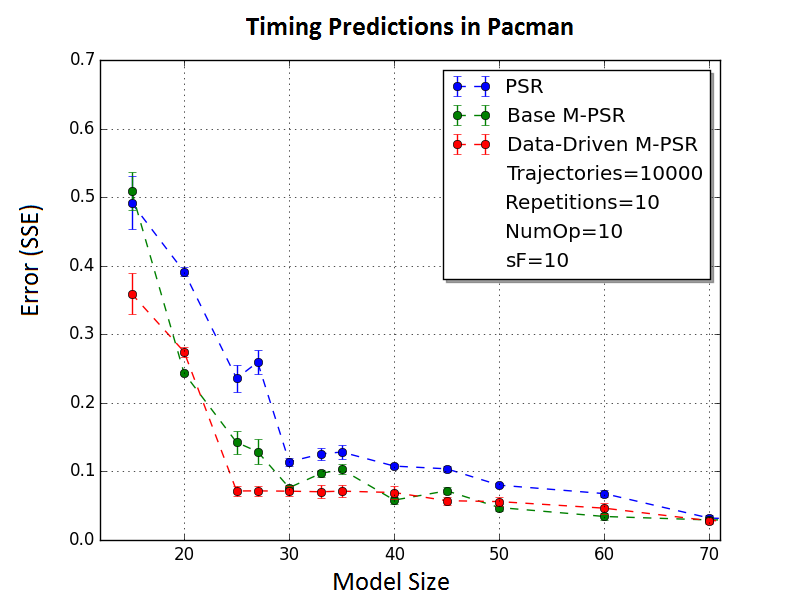
\includegraphics[width=\textwidth]{figs/Pacman/Pacman10k.png}
      \end{subfigure}
      ~
      \begin{subfigure}{1.1\textwidth}
        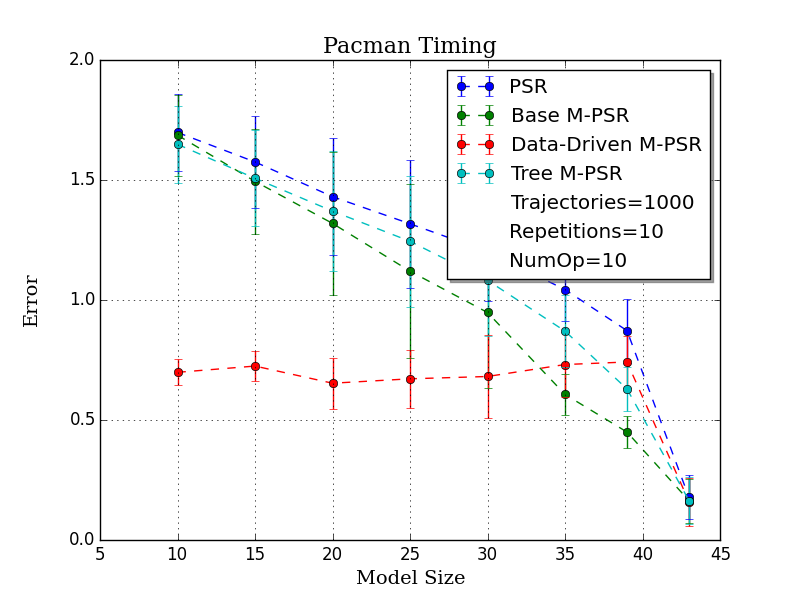
\includegraphics[width=\textwidth]{figs/DLMO/MO_1k.png}
      \end{subfigure}
      ~
      %\begin{subfigure}[b]{0.48\textwidth}
      %  \includegraphics[width=\textwidth]%{figs/DL/doubleLoopImage.png}
        %\caption{}
      %\end{subfigure}
      %~
      %\begin{subfigure}[b]{0.48\textwidth}
      %  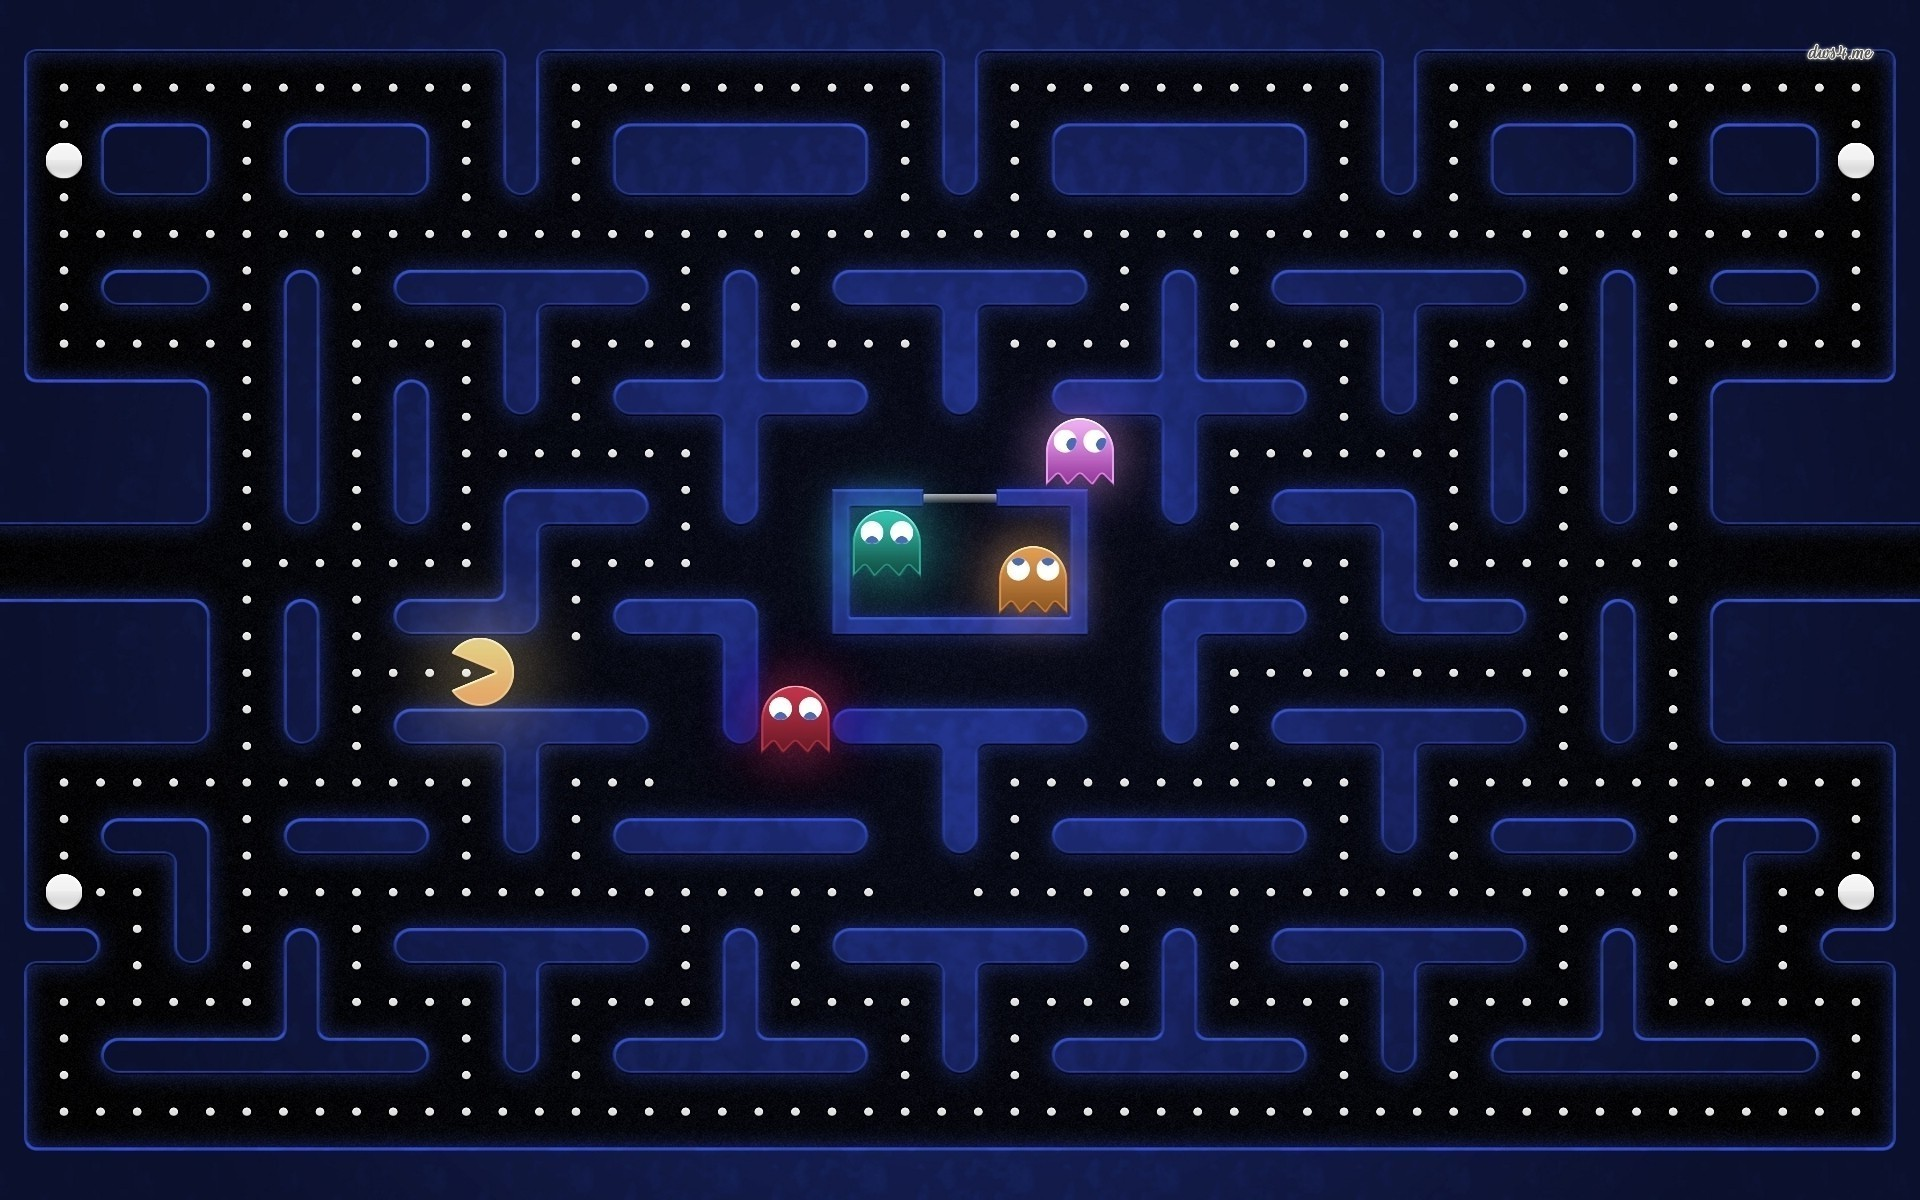
\includegraphics[width=\textwidth]{pac-man.jpg}
      %  \caption{}
      %\end{subfigure}
       %~
      %\begin{subfigure}[b]{0.33\textwidth}
        %
\includegraphics[height=11cm,width=9cm{figs/Pacman/graphPacMan.png}
        %\caption{}
      %\end{subfigure}
      
  \end{figure}
\end{block}
\vspace{-4.4ex}

\begin{block}{Conclusion}

M-PSRs offer large improvements over traditional PSRs when using smaller model sizes, as is often desired in practice. These improvements offer various prospects for future work:

\begin{itemize}
  \item Applications: planning, physiological signal recordings, and financial time-series
  \item Further optimization of the encoding function: $\kappa$, and selection of transition operators: $\Sigma'$
  \item Theoretical analysis of M-PSRs
\end{itemize}

\end{block}

%\begin{block}{References}

%\citep{balle2013spectral} % Insert publications even if they are not cited in the poster
%\citep{boots2010closing}
%\citep{pierrelucplanning2015}
%\small{\bibliographystyle{unsrt}
%\bibliography{sample}\vspace{0.75in}}
%\bibliographystyle{abbrv}
%\bibliography{sigproc}

%\end{block}

%----------------------------------------------------------------------------------------
%	REFERENCES
%----------------------------------------------------------------------------------------

%\begin{block}{References}

%\nocite{*} % Insert publications even if they are not cited in the poster
%\small{\bibliographystyle{unsrt}
%\bibliography{sample}\vspace{0.75in}}

%\end{block}

%----------------------------------------------------------------------------------------
%	ACKNOWLEDGEMENTS
%----------------------------------------------------------------------------------------

%\setbeamercolor{block title}{fg=red,bg=white} % Change the block title color

%\begin{block}{Acknowledgements}

%\small{\rmfamily{Nam mollis tristique neque eu luctus. Suspendisse rutrum congue nisi sed convallis. Aenean id neque dolor. Pellentesque habitant morbi tristique senectus et netus et malesuada fames ac turpis egestas.}} \\

%\end{block}

%----------------------------------------------------------------------------------------
%	CONTACT INFORMATION
%----------------------------------------------------------------------------------------

%\setbeamercolor{block alerted title}{fg=black,bg=norange} % Change the alert block title colors
%\setbeamercolor{block alerted body}{fg=black,bg=white} % Change the alert block body colors

%\begin{alertblock}{Contact Information}

%\begin{itemize}
%\item Web: \href{http://www.university.edu/smithlab}{http://www.university.edu/smithlab}
%\item Email: \href{mailto:john@smith.com}{john@smith.com}
%\item Phone: +1 (000) 111 1111
%\end{itemize}

%\end{alertblock}

%\begin{center}
%\includegraphics[width=0.6\linewidth]{mcgill.pdf} %& \hfill & 
\includegraphics[width=0.3\linewidth]{rllab.pdf}
%\end{center}

%----------------------------------------------------------------------------------------

\end{column} % End of the third column

\end{columns} % End of all the columns in the poster

\end{frame} % End of the enclosing frame

\end{document}
